\section{Additional Results}
\label{ssec:allresults}

Table~\ref{tab:confintmain} displays the point estimates from all estimators as well as confidence intervals calculated either (a) leave-one-state-out jackknife on the adjusted dataset (``CI (states)''); (b) leave-one-state-out jackknife repeating the entire adjusted leaving each state out (``CI (proc)''). This table also includes all analyses calculated on a second version of the adjusted data where we model a separate $\kappa$ for all values (heterogeneous). The confidence intervals are identical for ``None'' because this is the unadjusted dataset. ``Homogeneous'' is our preferred covariate adjustment, and the results presented in the main paper.

\begin{table}[h!]
\centering
\begin{threeparttable}
\caption{Point estimates and confidence intervals: primary dataset}
\label{tab:confintmain}
\begin{tabular}{llrll}
  \hline
Weight type & Adjustment & $\hat{\psi}$ & CI (states) & CI (proc) \\ 
  \hline
H-SBW & Homogeneous & -2.33 & (-3.49, -1.16) & (-3.47, -1.19) \\ 
  H-SBW & Heterogeneous & -2.24 & (-3.23, -1.24) & (-3.40, -1.08) \\ 
  H-SBW & No adjustment & -2.34 & (-2.85, -1.82) & (-2.85, -1.82) \\ 
  BC-HSBW & Homogeneous & -2.05 & (-3.27, -0.82) & (-3.22, -0.87) \\ 
  BC-HSBW & Heterogeneous & -1.98 & (-3.20, -0.76) & (-3.13, -0.83) \\ 
  BC-HSBW & No adjustment & -2.22 & (-2.87, -1.56) & (-2.87, -1.56) \\ 
  SBW & Homogeneous & -2.35 & (-3.65, -1.06) & (-3.67, -1.03) \\ 
  SBW & Heterogeneous & -2.28 & (-3.33, -1.22) & (-3.50, -1.05) \\ 
  SBW & No adjustment & -2.39 & (-2.95, -1.83) & (-2.95, -1.83) \\ 
  BC-SBW & Homogeneous & -2.07 & (-3.17, -0.97) & (-3.07, -1.06) \\ 
  BC-SBW & Heterogeneous & -2.00 & (-2.98, -1.01) & (-3.00, -0.99) \\ 
  BC-SBW & No adjustment & -2.19 & (-2.90, -1.49) & (-2.90, -1.49) \\ 
   \hline
\end{tabular}
    \begin{tablenotes}
      \item[] Note: The column ``CI (states)'' reflects the confidence interval from the jackknife procedure that conditions on the covariate adjustment procedure. The column ``CI (proc)'' accounts for the additional uncertainty of the covariate adjustment and recomputes the adjustment excluding each state.
    \end{tablenotes}
\end{threeparttable}
\end{table}

Table~\ref{tab:confintmainc2} presents the same results when excluding the early expansion states.

\begin{table}[h!]
\centering
\begin{threeparttable}
\caption{Point estimates and confidence intervals: early expansion excluded}
\label{tab:confintmainc2}
\begin{tabular}{llrll}
  \hline
Weight type & Adjustment & $\hat{\psi}$ & CI (states) & CI (proc) \\ 
  \hline
H-SBW & Homogeneous & -2.09 & (-2.85, -1.33) & (-3.15, -1.03) \\ 
  H-SBW & Heterogeneous & -2.06 & (-2.91, -1.22) & (-3.26, -0.87) \\ 
  H-SBW & No adjustment & -2.28 & (-2.82, -1.74) & (-2.82, -1.74) \\ 
  BC-HSBW & Homogeneous & -1.94 & (-2.96, -0.92) & (-3.17, -0.72) \\ 
  BC-HSBW & Heterogeneous & -1.93 & (-3.10, -0.76) & (-3.42, -0.45) \\ 
  BC-HSBW & No adjustment & -2.22 & (-3.07, -1.38) & (-3.07, -1.38) \\ 
  SBW & Homogeneous & -2.05 & (-2.75, -1.35) & (-3.10, -1.00) \\ 
  SBW & Heterogeneous & -2.03 & (-2.77, -1.29) & (-3.24, -0.82) \\ 
  SBW & No adjustment & -2.21 & (-2.71, -1.72) & (-2.71, -1.72) \\ 
  BC-SBW & Homogeneous & -1.99 & (-3, -0.99) & (-3.22, -0.77) \\ 
  BC-SBW & Heterogeneous & -2.00 & (-3.09, -0.9) & (-3.52, -0.47) \\ 
  BC-SBW & No adjustment & -2.23 & (-3.05, -1.40) & (-3.05, -1.40) \\ 
   \hline
\end{tabular}
    \begin{tablenotes}
      \item[] Note: The column ``CI (states)'' reflects the confidence interval from the jackknife procedure that conditions on the covariate adjustment procedure. The column ``CI (proc)'' accounts for the additional uncertainty of the covariate adjustment and recomputes the adjustment excluding each state.
    \end{tablenotes}
\end{threeparttable}
\end{table}

Figure~\ref{fig:loostateplot} displays the change in our estimator when removing each state for all four of our estimators on the adjusted dataset (``homogeneous'') and the unadjusted dataset (``none''). These results condition on the covariate adjustment, but are similar when recalculating the entire adjustment procedure. Additional results are available on request.

\begin{figure}[H]
\begin{center}
    \caption{Leave-one-state-out point estimates minus primary estimate}
    \label{fig:loostateplot}
    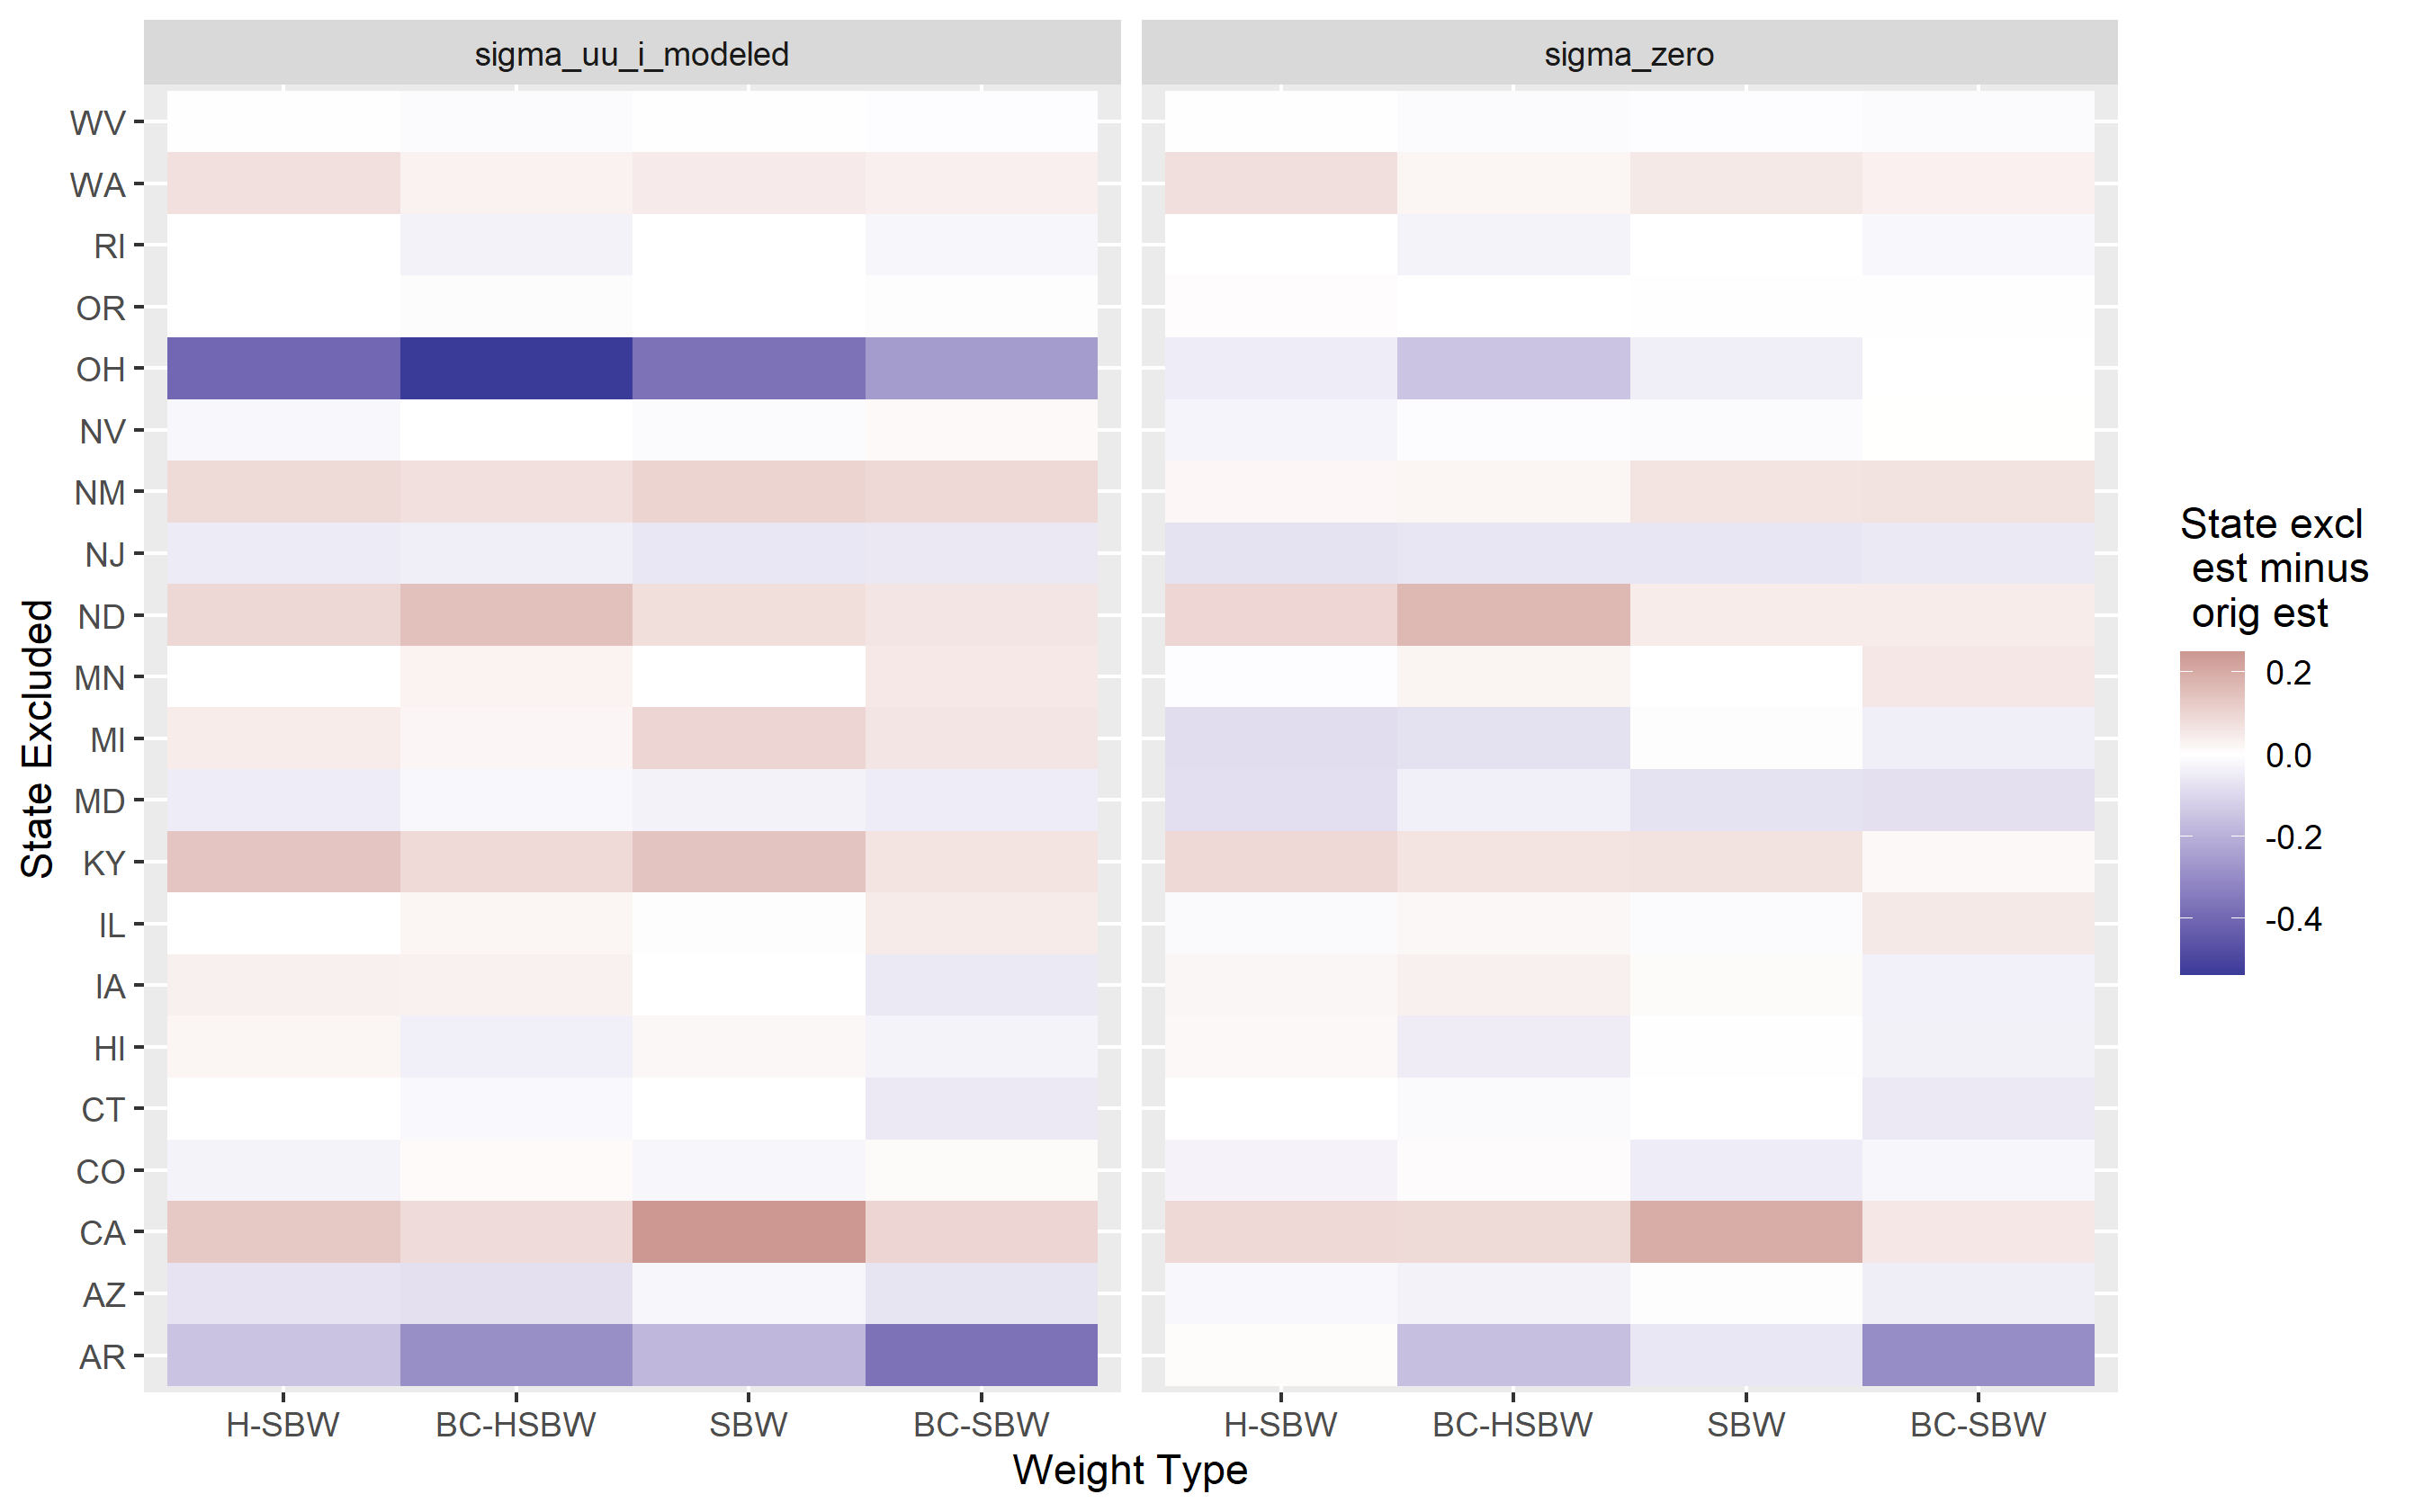
\includegraphics[scale=0.6]{01_Plots/loostate-sensitivityc1-state-uu-i.png}
\end{center}
\subcaption{Colors reflect the magnitude of the difference in the estimates when subtracting the original estimate from the estimate that excludes the specified state. The values in the left panel are conditional on homogeneous covariate adjustment. The values in the right panel are on the unadjusted data.}
\end{figure}

\clearpage
